\documentclass[10pt,compress,serif,aspectratio=169]{beamer}
\usepackage{pres2023_169}
\usepackage[utf8]{inputenc}
\graphicspath{{figures/}}
 
\author[JTCAM]{G. Anciaux}
%
\title[JTCAM]{Why not \textit{Diamon Open Access} ?}

\begin{document}

\maketitle

%\usebackgroundtemplate{
\includegraphics[width=12.8cm,height=9.6cm]{cover2.pdf}}{\begin{frame}[t,plain]\end{frame}}
% %%%%%%%%%%%%%%%%%%%%%%%%%%%%%%%%%%%%%%%%%%%%%%%%%%%%%%%%%%%%%%%%%%%%%%%%%%%%%%%%%%


%\usebackgroundtemplate{
\includegraphics[height=10cm]{bg.pdf}}

%%%

\begin{frame}[t]%
 \titleframe{History}\vskip1cm%

{\large First scientific press:\newline}
 
 \begin{itemize}


 \item 1450: Printing Press (in europe)
 \item 1534: Foundation of Cambridge University Press
   %Foundation of Cambridge University Press, the oldest university press and publishing house in the world
 \item 1665: \textit{Journal des Sçavans} (France), \textit{Philosophical Transactions of the Royal Society} (UK)\\
   %Creation of Le Journal des Sçavans in France, the first academic journal. Soon after, the Philosophical Transactions of the Royal Society appears in the UK. It still exists today[5]. The familiar functions of the scientific journal –registration, certification, dissemination, and archiving– are already present[6]
 \end{itemize}

 \vfill
{\large Yet defined the purpose of scientific journals:\newline}

\begin{itemize}
\item registration: authorship/priority claim
\item certification: usually peer-review
\item dissemination: provide (targeted) access
\item archiving: permanent access link (citable) 
\end{itemize}
\end{frame}

 %%%
\begin{frame}[t]%
 \titleframe{Author and Copy rights}\vskip1cm%
\begin{itemize}

 \item 1710: \textit{Statute of Anne}: British authors can control the copying of their books 
   % Royal assent to the Statute of Anne. The British authors are granted the right to control the copying of their books. The duration of copyright is 14 years(renewable once), after which the books enter the public domain[7]. This new regime follows a period of censorship and monopoly(by the Stationer’s Company) and a period of no regulation, which called for a new licensing protecting the authors
 \item 1852: articles published (in FR/UK) can be freely reprinted and translated (unless reserved rights are explicitly mentioned)
   % Signature of a bilateral treaty between the UK and France: all articles published abroad in periodicals can be freely reprinted and translated, unless reserved rights are explicitly mentioned[8]
 \item Foundation of Nature (1869) and Elsevier (1880)
   %Foundation of the British scientific journal Nature[9]
 %1880: Foundation of the Dutch publishing company Elsevier[10]
 \item 1886: Berne Convention governing copyright: grants a CC BY licence by default.%Signature of the Berne Convention, an international agreement governing copyright. Its article 7 states: “Articles from newspapers or periodicals published in any of the countries of the Union may be reproduced in original or in translation in other countries of the Union, unless the authors or publishers have expressly forbidden it.” [11] In today’s parlance, the Berne Convention grants a CC BY licence by default.

 \item 1908: Berlin Act reverses the standards: reproduction implicitly forbidden. %1908: Berlin Act: revision of the Berne Convention. It reverses the standards: instead of being implicitly allowed, reproduction is now implicitly forbidden. Its article 9 states: “Serial stories, tales, and all other works, whether literary, scientific, or artistic, whatever their object, published in the newspapers or periodicals of one of the countries of the Union, may not be reproduced in the other countries without the consent of the authors.” The Berne convention has later been further updated, but this restriction remains. Most countries have now signed it [11].
 \item 1928: Rome Act: author’s rights $\neq$ copyright
   %1928: Rome Act: revision of the Berne Convention. The article 6bis states: “Independently of the author’s copyright, and even after transfer of the said copyright, the author shall have the right to claim authorship of the work, as well as the right to object to any distortion, mutilation or other modification of the said work which would be prejudicial to his honour or reputation.”. This implements the moral rights of the authors, which is an essential feature of the author’s rights or droit d’auteur, as opposed to the copyright.
 \end{itemize}
\end{frame}

 %%%

\begin{frame}[t]%
 \titleframe{History}\vskip1cm%
{
 \begin{center}
   \Large Post-World War II\\ Research budgets increase enormously
 \end{center}
}
\only<1>{
 \begin{quote}The average yearly growth of the US federal budget dedicated to non-defense R\&D between 1953 and 1973 is more than 15\% [12].
 \end{quote}
}

\only<2>{
 \begin{center}
 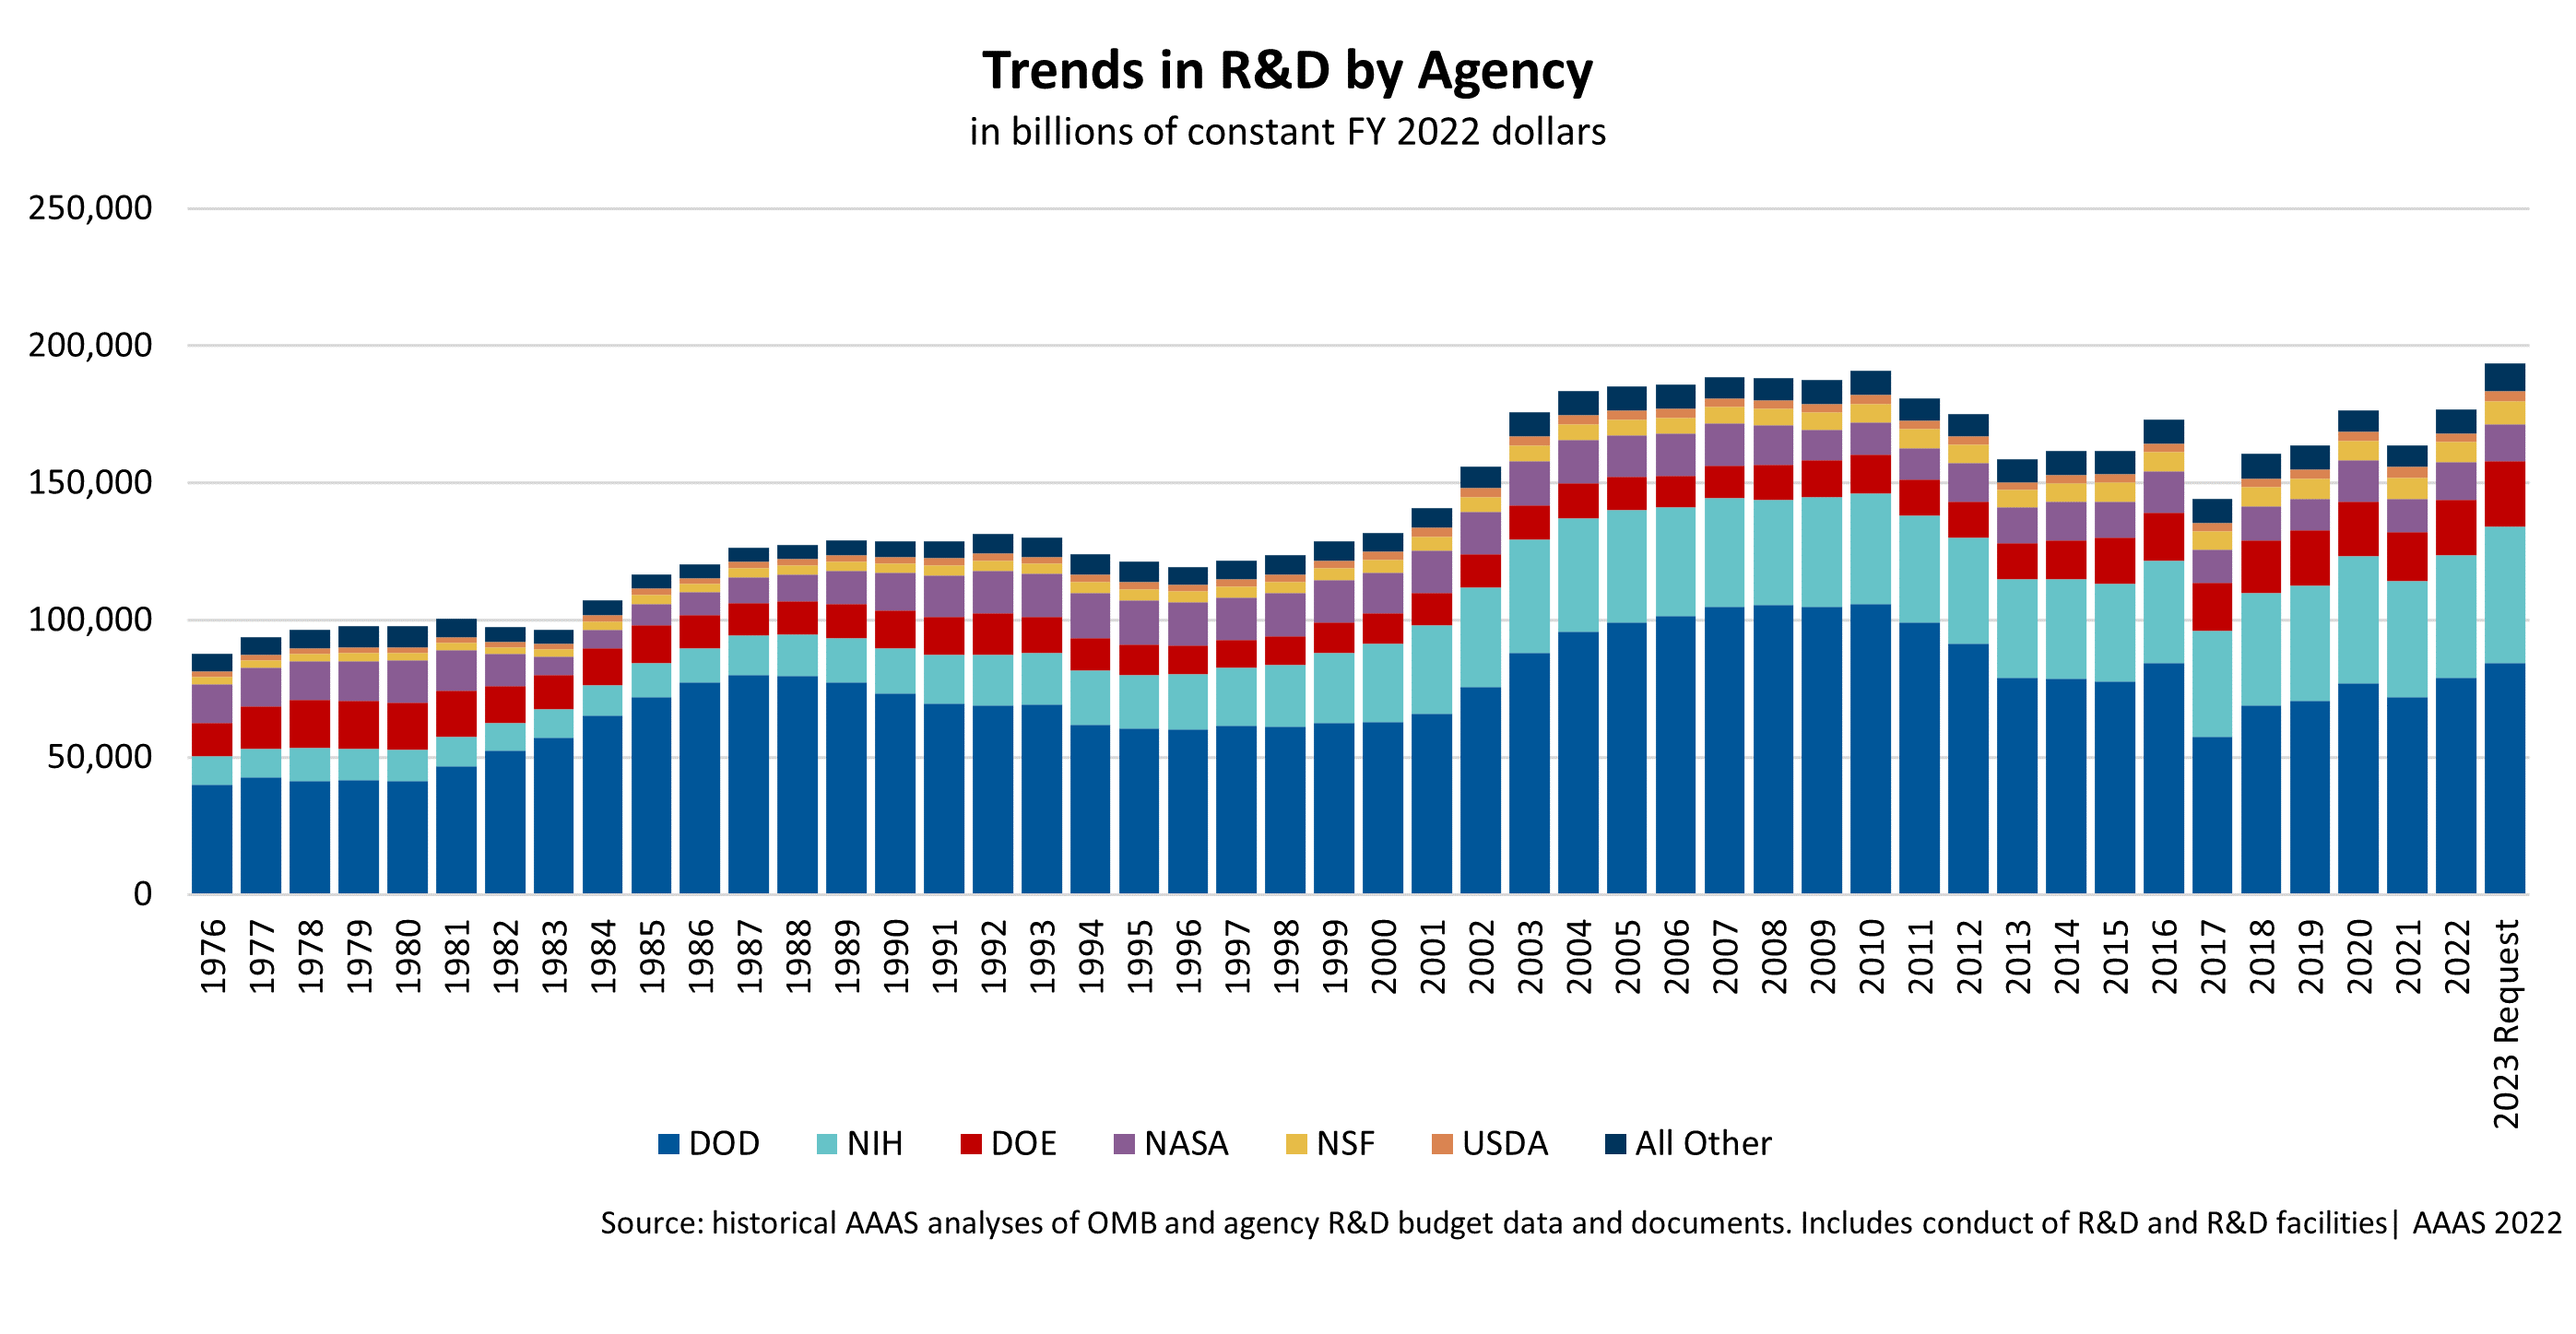
\includegraphics[width=\textwidth]{Agencies.png}
\end{center}
}
\only<3>{
 \begin{center}
 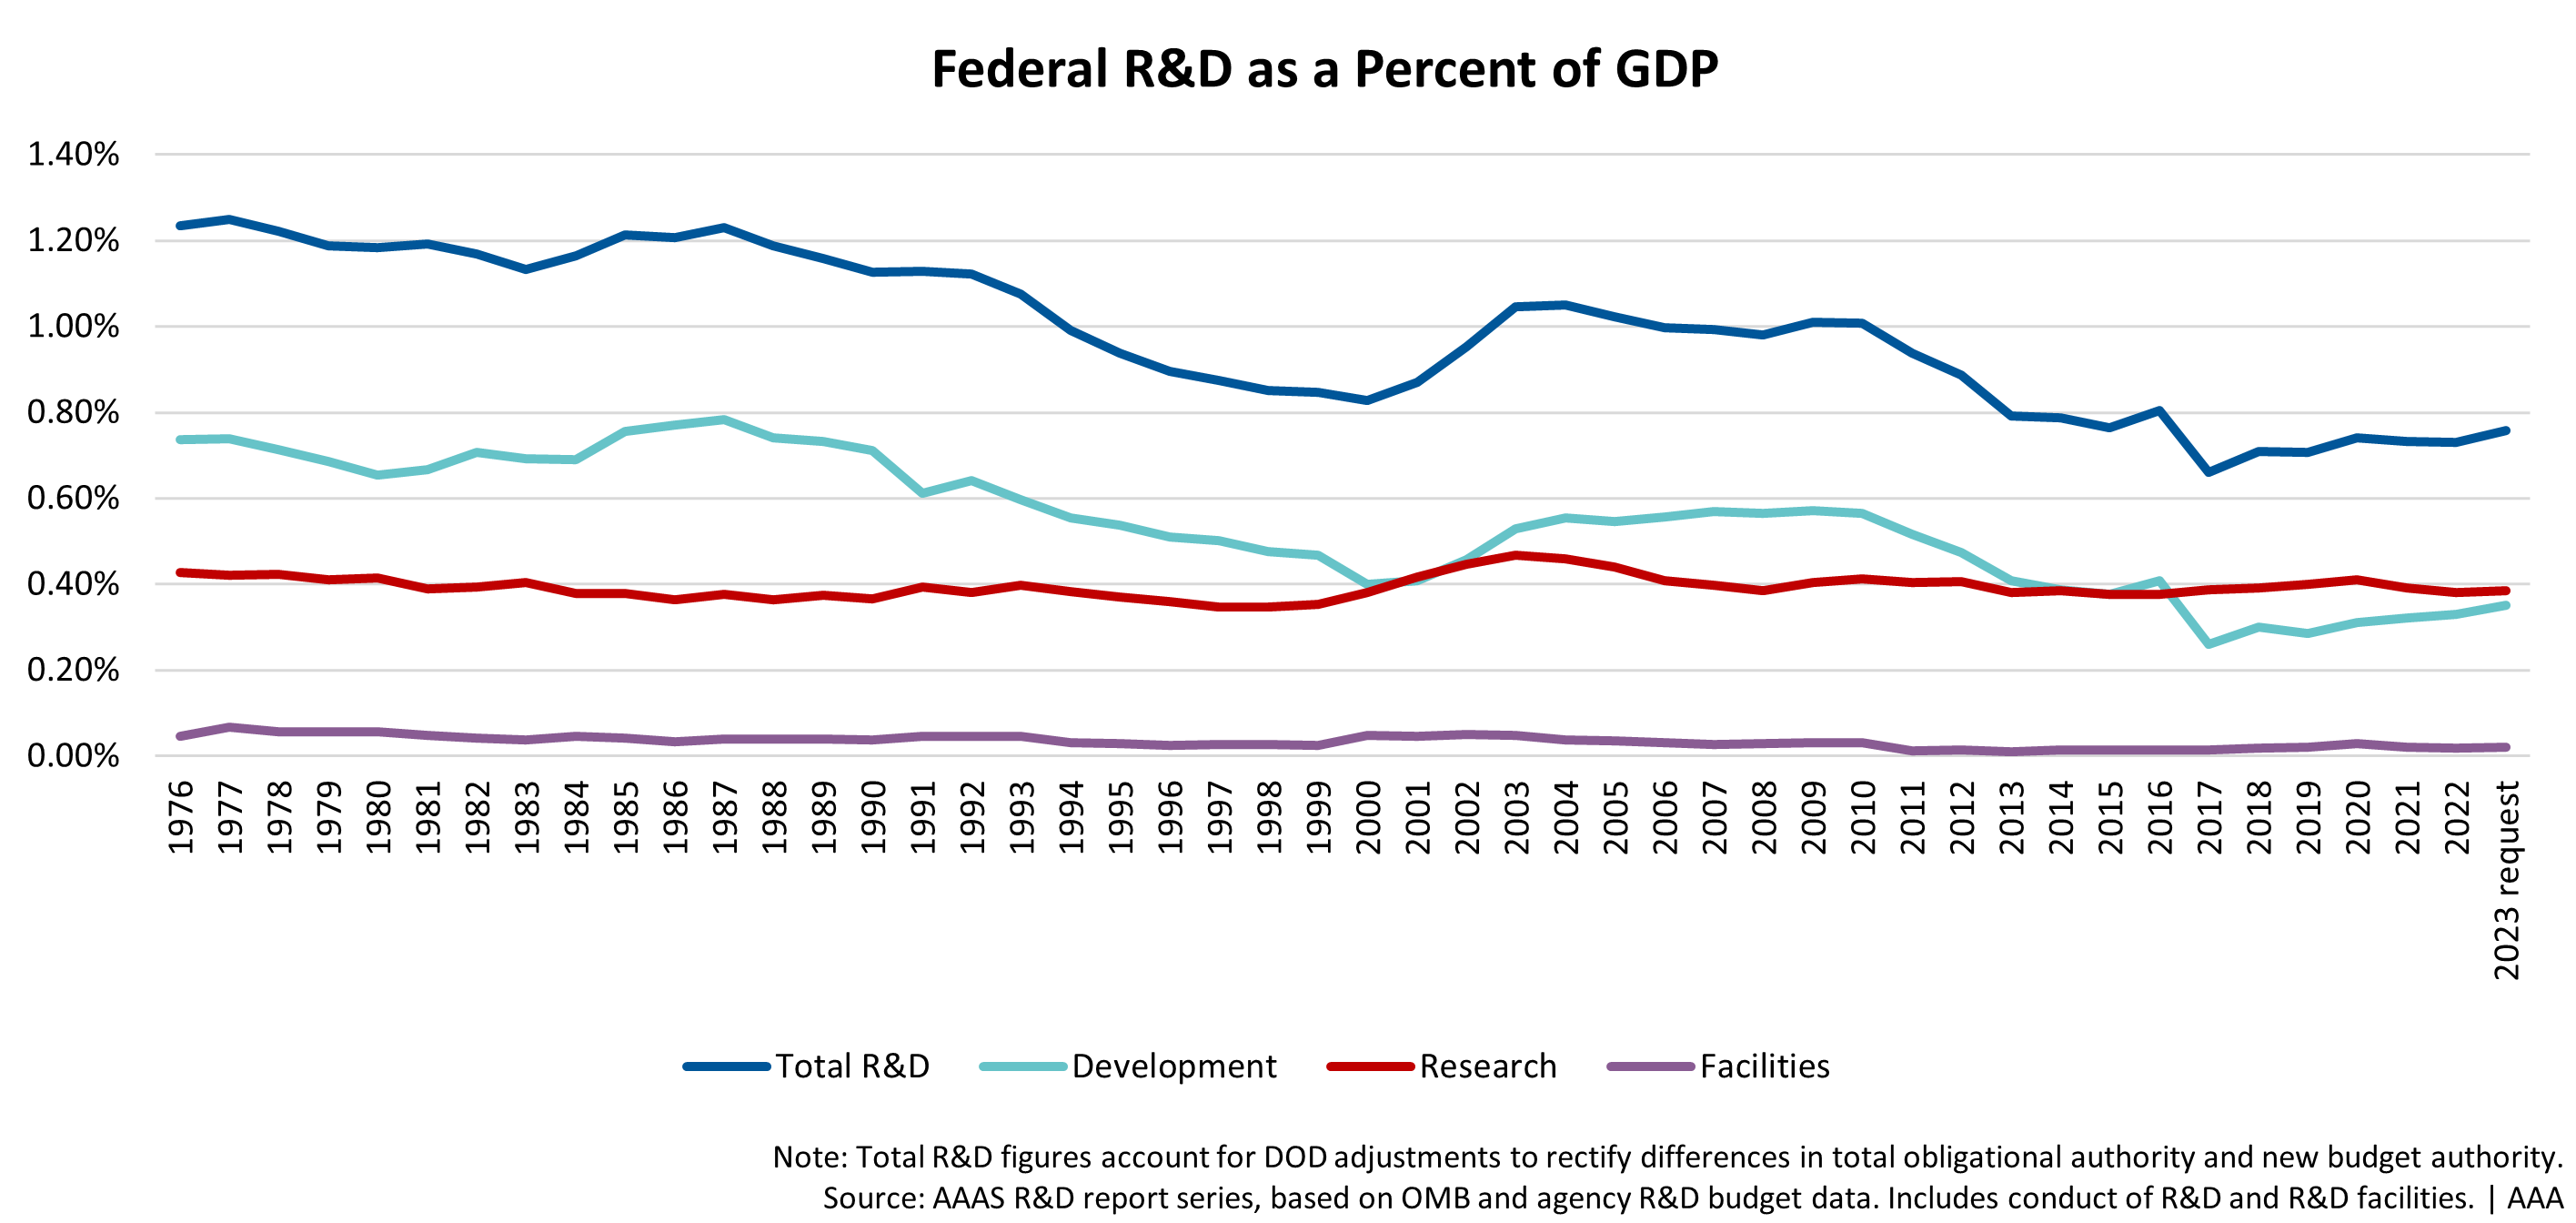
\includegraphics[width=\textwidth]{RDGDP.png}
\end{center}
}
\only<4>{
 \begin{center}
 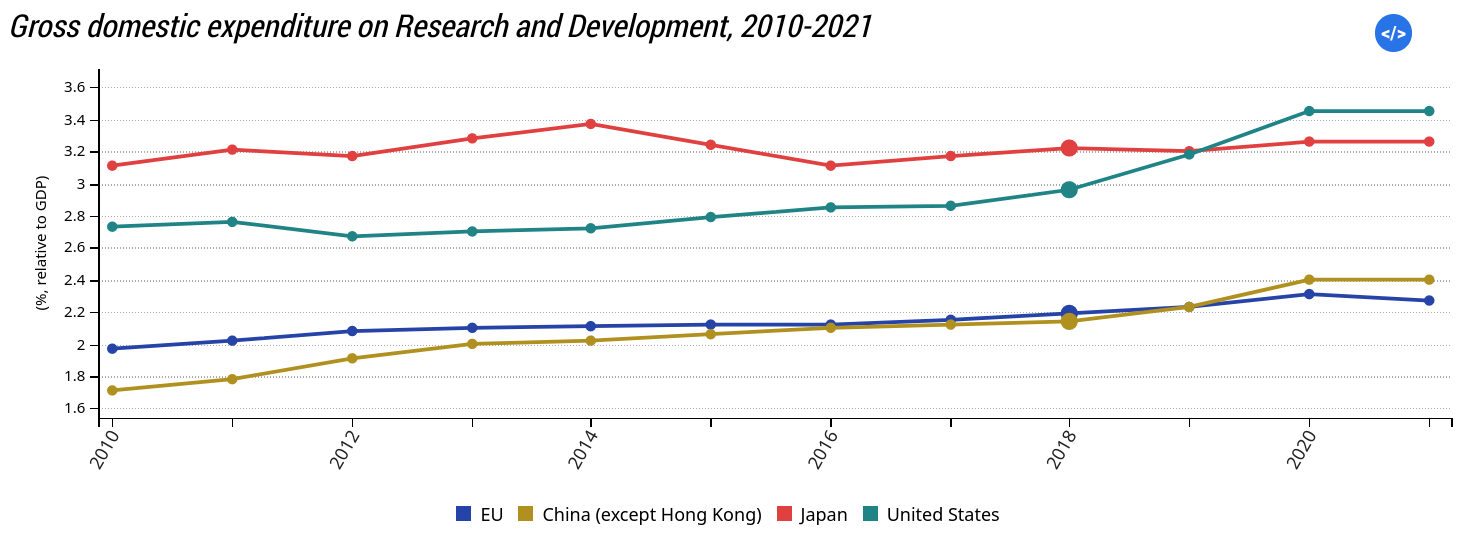
\includegraphics[width=\textwidth]{RDGDP-global.png}
\end{center}
}
 \end{frame}

 %%%
 
 \begin{frame}[t]%
 \titleframe{New scientific publishing mechanisms}\vskip1cm%
\begin{itemize}

 \item 1951: Pergamon Press (now \textbf{Elsevier}) and R. Maxwell: many new thematic journals
   %1951: Robert Maxwell creates Pergamon Press. Academic journals used to be mainly owned by learned societies. Maxwell perceives the potential huge profitability of academic publishing as the public funding for research rises. He creates many new journals for specific fields of research and surfs on globalisation with grand titles like ‘International Journal of’. Pergamon Press is sold to Elsevier in 1991. [13]
 \item 1955: appearance of \textbf{impact factor}
   % The idea of an impact factor is first mentioned by Eugene Garfield in Science. It was originally thought of as a tool for librarians to identify journals to purchase, not as a measure of the quality of research [14]. Since 1975, it has been computed and published in the Journal Citation Reports (JCR), nowadays owned by Clarivate [15].
 \item 1970s: rise of journals subscriptions $\Rightarrow$ emerging crisis
   % Beginning of the serials pricing crisis: the prices of subscriptions to scholarly journals rise tremendously. For instance, between 1973 and 1987, the average price increases by 12\% per year, while the costs for the publishers only rise increase by 8\% [16, p. 22]. This difference between expenses and revenue enables the publishers to make big margins. Librarians start to organise and fight back.
 \item 1991: creation free archive \textit{xxx.lanl.gov} at Los Alamos National Laboratory (to become \textbf{arXiv.org}).
% Paul Ginsparg creates the free archive xxx.lanl.gov at Los Alamos National Laboratory, which will become arXiv.org 10 years later [17].
\item By 1994, three years after acquiring Pergamon, Elsevier had raised its prices by 50\%. Librarians began cancelling subscriptions to less popular journals.
\end{itemize}
\end{frame}

 %%%
 
 \begin{frame}[t]%
 \titleframe{Open access models}\vskip1cm%
\begin{itemize}

\item 2000: Foundation of \textbf{BioMed Central} publisher (now in Springer Nature) and online open-access with \textbf{article processing charge (APC)}
 % Foundation of \textit{BioMed Central} publisher and by Vitek Tracz. This publisher inaugurates a business model based on online open-access journals with an article processing charge (APC). It is now part of Springer Nature. [18]
\item 2000: 34,000 scientists petition:
  \begin{quote}
    “we will publish in, edit and review for, and personally subscribe to only those scholarly and scientific journals that have agreed to grant unrestricted free distribution rights to any and all original research reports.”
  \end{quote}
  Leads to \textbf{the Public Library of Science (PLoS)}, with APC[19]

  \item 2002: \textbf{Budapest Open Access Initiative (BOAI)}: promotes open access \textbf{but} no recommendation for the costs
    %Budapest Open Access Initiative (BOAI). This landmark conference on the open access movement is organised by the Open Society Institute. It results in a public call to promote open access of scholarly literature, insisting on the need to remove all access fees for the readers, but it does not promote any particular model to cover the costs. [20]
  \item 2005: The Wellcome Trust foundation: \textbf{requires output open access}
    % The Wellcome Trust, a British research foundation, starts requiring open access for the research they fund. [21]
  \item 2018: \href{https://www.snf.ch/en/bQ17hb9mM1NC4awy/news/news-181010-make-open-access-the-new-normal}{SNF allows to budget OA APC}
  \item 2021: \href{https://www.coalition-s.org/}{The Plan/cOAlition S}: requires Open Access journals or platforms. Followed by \href{https://www.coalition-s.org/supporters/}{many institutions}
    %requires scientific publications resulting from research funded by public grants to be published in compliant Open Access journals or platforms. It is supported by major institutions such as the World Health Organization, the Bill \& Melinda Gates Foundation, the European Commission. [23]
 \end{itemize}
\end{frame}

%%% 

\begin{frame}[t]%
  \titleframe{Publication metrics}\vskip1cm%


  2013: \textbf{San Francisco Declaration on Research Assessment (DORA)}
  \begin{quote}“Do not use journal-based metrics, such as Journal Impact Factors, as a surrogate measure of the quality of individual research articles, to assess an individual scientist’s contributions, or in hiring, promotion, or funding decisions.”\end{quote}
   %The declaration is signed by more than 2400 organisations, including universities, funding agencies, and also publishers like Springer-Nature or Elsevier. [22]

\end{frame}
%%% 

   \begin{frame}[t]%
 \titleframe{Number of papers produced}\vskip1cm%

 In 2006: 50 million papers have been published since scholarly articles first appeared [5]. Over three centuries, the annual number of published articles has grown exponentially at a 3\% rate.

\end{frame}

%%%


\begin{frame}[t]%
 \titleframe{Open Access Models}\vskip1cm%

 
 \begin{itemize}
 \item Gold:
   \begin{itemize}
   \item Immediate open access publication
   \item created by the publisher
   \item made available by publisher online platform
   \item published under a licence that permits reuse (CC) licence.
   \end{itemize}
 \item Green (self-archiving):
   \begin{itemize}
   \item A version of the publication is archived online, e.g., in a repository (arXiv, HAL, infoscience).
   \item does not include the (publisher) work of copyediting, proofreading, typesetting, indexing, metadata tagging, marketing or distribution.
   \item Not listed by publishers (no metrics)
   \item can be freely accessed (with possible embargo period)
   \item Limited licencing
   \end{itemize}

 %\item Bronze
 %  \begin{itemize}
 %  \item free to read and/or download on the publisher’s website
 %  \item closed licence precluding sharing or re-use
 %  \item Authors do not retain the copyright (publisher can withdraw access and the book cannot be shared elsewhere)
 %  \end{itemize}
 %\item Grey
 %  \begin{itemize}
 %  \item Shared online by an academic on personal/social website (researchgate)
 %  \item Illegal if no open licence release nor a Green OA route
 %  \item Tolerated by editors?
 %  \end{itemize}
 %\item Black: Illegal publication

 \end{itemize}
 \vfill
\href{ https://oabooks-toolkit.org/lifecycle/article/13868103-green-gold-diamond-different-models-for-open-access-books}{Credits to oabooks-toolkit}

\end{frame} 
%%%

\begin{frame}[t]%
 \titleframe{SNF Open access recommendations}\vskip1cm%

 \begin{center}
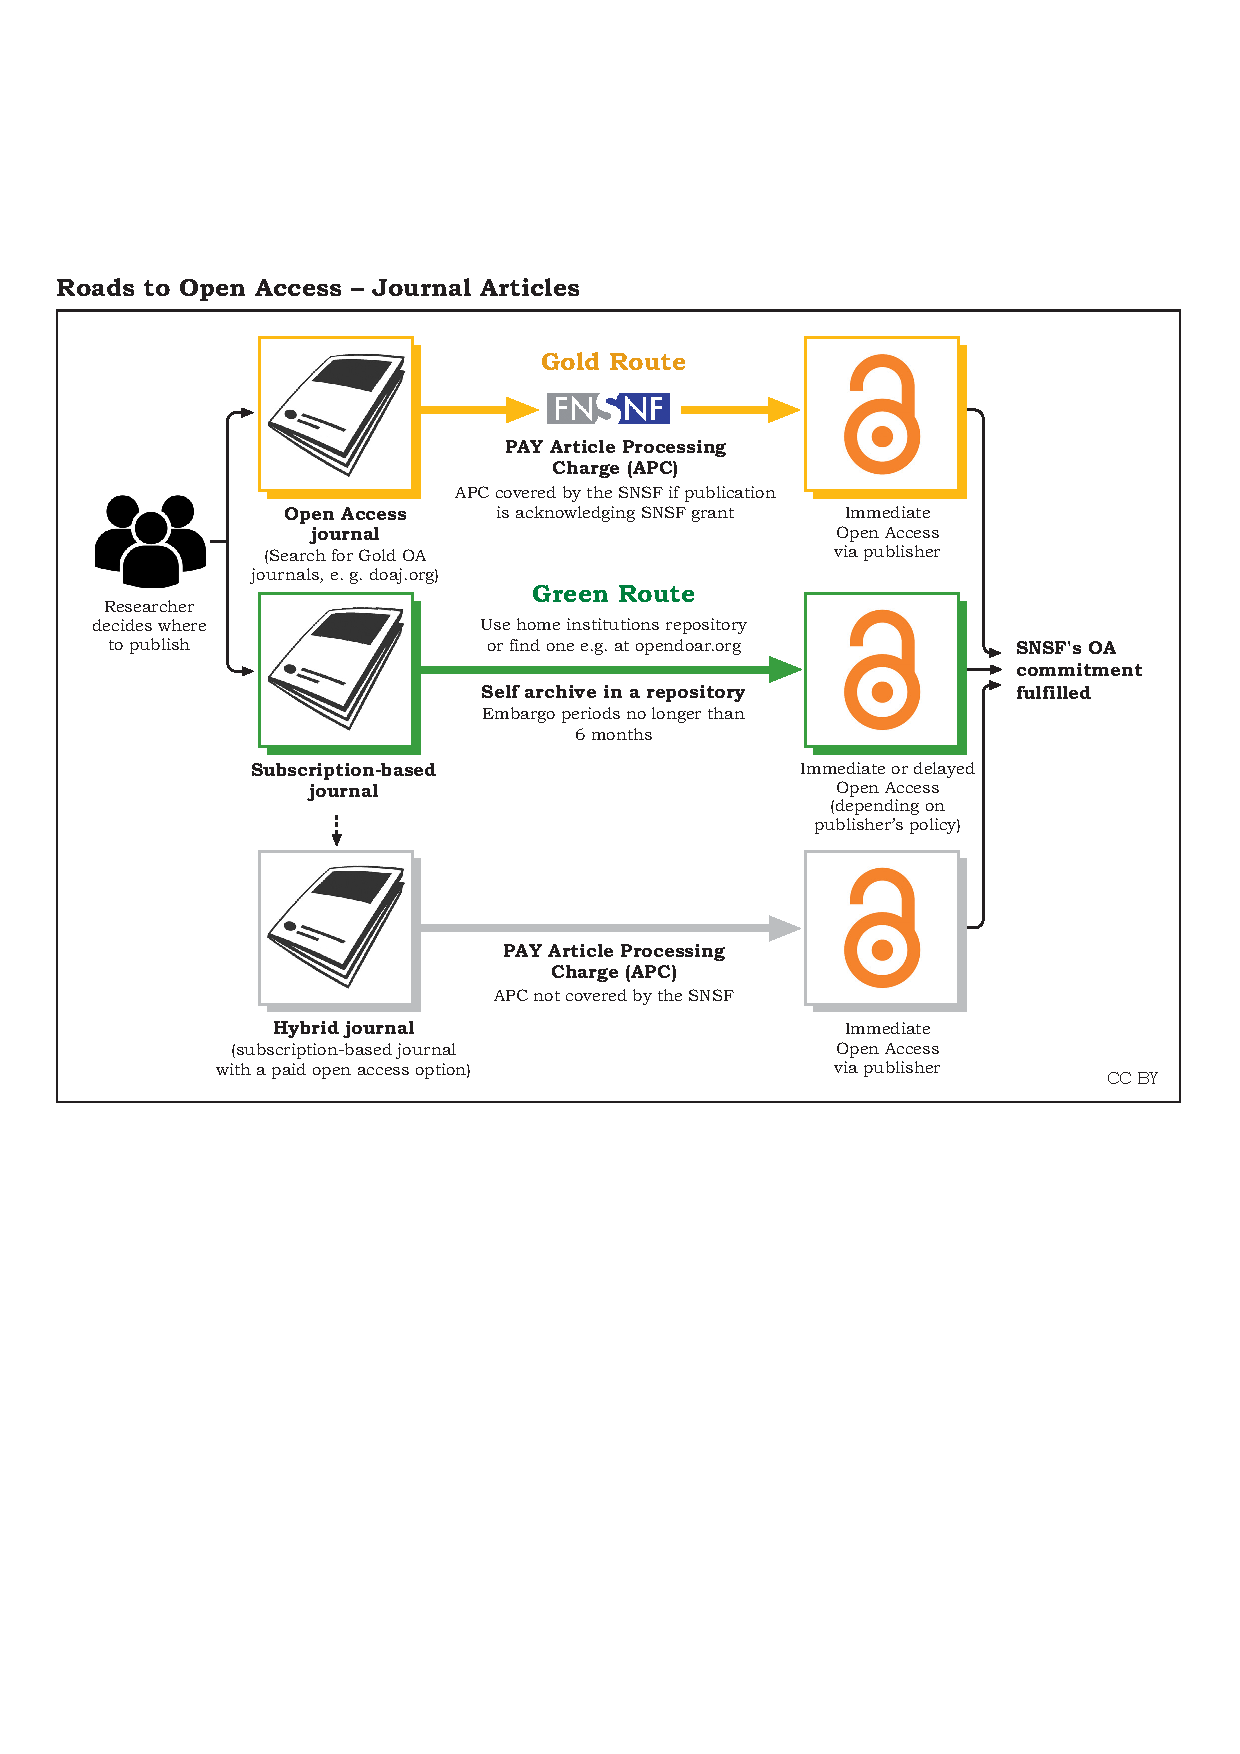
\includegraphics[width=.65\textwidth]{SNSF_Roads_to_OA_Articles}
\end{center}
\href{https://www.snf.ch/en/VyUvGzptStOEpUoC/topic/open-access-to-publications}{Illustration taken from www.snf.ch}

\end{frame}

%%% 


\begin{frame}[t]%
 \titleframe{What is the problem?}\vskip1cm%

S. Buranyi, \textit{Is the staggeringly profitable business of scientific publishing bad for science?}, The Guardian (2017)\\
{\tiny \url{https://www.theguardian.com/science/2017/jun/27/profitable-business-scientific-publishing-bad-for-science}}

%Scientists are well aware that they seem to be getting a bad deal. The publishing business is “perverse and needless”, the Berkeley biologist Michael Eisen wrote in a 2003 article for the Guardian, declaring that it “should be a public scandal”. Adrian Sutton, a physicist at Imperial College, told me that scientists “are all slaves to publishers. What other industry receives its raw materials from its customers, gets those same customers to carry out the quality control of those materials, and then sells the same materials back to the customers at a vastly inflated price?” (A representative of RELX Group, the official name of Elsevier since 2015, told me that it and other publishers “serve the research community by doing things that they need that they either cannot, or do not do on their own, and charge a fair price for that service”.)


Randy Schekman: “Despite my giving sermons all over the world on this topic, it seems journals hold sway even more prominently than before. It is that influence, more than the profits that drove the system’s expansion, that most frustrates scientists today.“

 Elsevier says its primary goal is to facilitate the work of scientists and other researchers. An Elsevier rep noted that the company received 1.5m article submissions last year, and published 420,000; 14 million scientists entrust Elsevier to publish their results, and 800,000 scientists donate their time to help them with editing and peer-review. “We help researchers be more productive and efficient,” Alicia Wise, senior vice president of global strategic networks, told me. “And that’s a win for research institutions, and for research funders like governments.”


 guardian:

 Whatever the fate of Sci-Hub, it seems that frustration with the current system is growing. But history shows that betting against science publishers is a risky move. After all, back in 1988, Maxwell predicted that in the future there would only be a handful of immensely powerful publishing companies left, and that they would ply their trade in an electronic age with no printing costs, leading to almost “pure profit”. That sounds a lot like the world we live in now.
\end{frame}



%%%

\begin{frame}[t]%
 \titleframe{Cost of a publication?}\vskip1cm%
\fig{.6}{publisher-shares}
\end{frame}

%%%

\begin{frame}[t]%
 \titleframe{Cost of a publication?}\vskip1cm%
 \fig{.6}{publishers-revenues}
 \begin{quote}
   Revenues in 2020 of the biggest publishers in \$ corresponding to the publishing segment only. MDPI figures are estimatations based on APC.
 \end{quote}
\end{frame}

%%%

\begin{frame}[t]%
 \titleframe{Cost of a publication?}\vskip1cm%
 \fig{.6}{publisher-margins}
 \begin{quote}
   \small
Operating margins in 2020 in \%. The operating margin is the ratio of the operating income (or profit) with the revenue. Taylor \& Francis, Elsevier and Wiley publish an adjusted operating income which includes some technical corrections without changing the value substantially. Springer Nature does not publish its operating profit because its shares are not traded on the stockexchange.  
 \end{quote}
\end{frame}

%%%
\begin{frame}[t]%
 \titleframe{Cost of a publication?}\vskip1cm%

\href{https://doi.org/10.12688/f1000research.27468.2}{Grossmann, A. \& Brembs, B. Current market rates for scholarly publishing services. (2021)} 
\begin{quote}
  \vspace{.5cm}
   [...] conservative estimates show that the publication cost for a representative scholarly article \textbf{is around \$400}.
 \end{quote}

 \pause
 \vfill
\centering{
 \Large{How to evaluate such a cost?}}
\end{frame}

%%%

\begin{frame}[t]%
 \titleframe{Cost of a publication?}\vskip1cm%

 \begin{minipage}{.45\textwidth}
   Content acquisition
   \begin{itemize}
   \item Authors (re-)submission
   \item Dealing with reviewers
   \item Plagiarism/Similarity check
   \item DOI for paper\&reviews
   \item APC collection
   \end{itemize}
 \end{minipage}
 \hfill
   \pause
 \begin{minipage}{.45\textwidth}
   Content preparation
   \begin{itemize}
   \item Manuscript tracking
   \item Production check-in
   \item Manuscript Technical checking
   \item Copyediting, Typesetting, Figures/graphs/tables
   \item Metadata, metrics
   \item Authors corrections
   \end{itemize}
\end{minipage}
\vfill
\pause
\begin{center}
 \begin{minipage}{.7\textwidth}
  Dissemination/archiving
  \begin{itemize}
  \item Web OA platform and hosting
  \item Long-term digital preservation
  \item Distribution to indexing services (Scopus, PMC, DOAJ, ...)
  \end{itemize}
\end{minipage}
\end{center}
%\begin{minipage}{.45\textwidth}
% \end{minipage}
\end{frame}


%%%
\begin{frame}[t]%
 \titleframe{Cost of a publication?}\vskip1cm%

 \begin{center}
 \alert{\Large Yet APC's are ...}\\
 \end{center}

 \pause
 \fig{.7}{publisher-APC}
\end{frame}

%%%

\begin{frame}[t]%
 \titleframe{Diamond Open Access}\vskip1cm%

Wikipedia Definition:\newline \newline
 \begin{quote}
   \textbf{Diamond open access} refers to academic texts (such as monographs, edited collections, and journal articles) published/distributed/preserved with \textbf{no fees to either reader or author.} \newline
 \end{quote}
 \pause
\href{https://doi.org/10.5281/zenodo.4558704}{OA Diamond Journals Study. Part 1: Findings. (2021)\newline}

\textbf{Landscape}\\
\begin{itemize}
\item $\sim 29000$ DOA journals (30\% in DOAJ)
\item Fewer articles (356000 per year vs. 453000 APC ones), average $\sim$ 25 articles/year
\item Since 2018 $\searrow$ DOA articles while $\nearrow$ of APC-ones
\item 45\% in Europe, 25\% in Latin America, 16\% in Asia, 5\% in the US/Canada
\item 60\% HSS, 22\% science, 17\% medicine
\end{itemize}

\end{frame}

%%%

\begin{frame}[t]%
 \titleframe{Diamond Open Access}\vskip1cm%

Wikipedia Definition:\newline \newline
 \begin{quote}
   \textbf{Diamond open access} refers to academic texts (such as monographs, edited collections, and journal articles) published/distributed/preserved with \textbf{no fees to either reader or author.} \newline
 \end{quote}

\href{https://doi.org/10.5281/zenodo.4558704}{OA Diamond Journals Study. Part 1: Findings. (2021)\newline}

\textbf{Sustainability and funding}\\
\begin{itemize}
  \item 60\% of DOA journals depend on volunteers
  \item The majority (53\%) run with less than 1 FTE
  \item 70\% declared less than \$/€10,000 annual costs.
  \item Funding mainly by Universities, and much less by Funding agencies
\end{itemize}
\end{frame}

%%%

\begin{frame}[t]%
 \titleframe{Diamond open in CH}\vskip1cm%


 1. Projet PLATO: l’Open Access Diamant est en bonne voie en Suisse - Bibliothèque - UNIGE. https://www.unige.ch/biblio/fr/actus/projet-plato/ (2023).
\end{frame}

%%% 

\begin{frame}[t]%
 \titleframe{What is an Overlay Journal?}\vskip1cm%
 \begin{center}%
   \only<1>{\fig{1}{epirevue_0d}}%
   \only<2>{\fig{1}{epirevue_1d}}%
   \only<3>{\fig{1}{epirevue_2d}}%
    \only<4>{\fig{1}{epirevue_3d}}%
   \only<5>{\fig{1}{epirevue_4d}}%
   \only<6>{\fig{1}{epirevue_5d}}%
 \end{center}%
\end{frame}
 
%%%

\begin{frame}[t]
 \titleframe{Motivation \& Chronology}\vskip0.6cm

{\centering$\to$\;\textbf{To offer an ethical and open publication model}}\\[1em]

%\textbf{Historique}
 \begin{itemize}
  \item \parbox{1.5cm}{2015/09} First discussion between VA \& ML\\[.5em]
  \item \parbox{1.5cm}{2017/07} Online discussion with interested contributors\\[.5em]
  \item \parbox{1.5cm}{2018/05} Steering committee (title, logo, etc)\\[.5em]
  \item \parbox{1.5cm}{2019/06} Scientific committee (25 members)\\[.5em]
  \item \parbox{1.5cm}{2020/01} JTCAM accepted by the Episciences plateform\\[.5em]
  \item \parbox{1.5cm}{2020/05} Editorial committee (10 members)\\[.5em]
  \item \parbox{1.5cm}{2020/08} Official JTCAM kick-off\\[.5em]
  \item \parbox{1.5cm}{2020/09} First submission
  \item \parbox{1.5cm}{2022/10} Referenced in DOAJ
 \end{itemize}

\end{frame}

%%%

\begin{frame}[t]
\titleframe{Research Community}\vskip0.6cm
\begin{itemize}
 \item Solid Mechanics
 \item Not well aware of Open Access good practices
 \item Wide spectrum: theoretical, applied, numerical, experimental
 \item Classical journals and publishers
 \begin{itemize}
 \item IJP, JMPS, IJSS, CMAME, IJMM, TI, IJES, Wear, ActaMat (Elsevier)
 \item IJNME, Adv Mat (Wiley)
 \item Comp Mech, Meccanica (Springer)
 \item PRS (Cambridge)
 \item Mechanics of Adv Mat and Struct (Taylor \& Francis)
 \end{itemize}
 \item Alternate journals (Diamond Open Access)
  \begin{itemize}
 \item CRAS (Mersenne)
 \item Archives of Mechanics (since 1950)
 \item Technische Mechanik
 \item Mathematics and Mechanics of Complex Systems (half-diamond)
 \item JACM
 \item ACM
 \end{itemize}
\end{itemize}

\end{frame}

%%%

\begin{frame}[t]
 \titleframe{JTCAM specific features}\vskip0.6cm
 \begin{itemize}
  \item \textbf{Overlay Journal}
  \begin{itemize}
  \item Always a preprint shared on Open Archives (even for refused papers)
  \item Diamond Open Access
  \end{itemize}
  \item \textbf{Team}
  \begin{itemize}
  \item Technical board: creators of the journal + data/software editor
  \item Scientific Board: invited
  \item Editorial board: elected
  \item Collegial decisions, no editor in chief
  \end{itemize}
	\item\textbf{Open Review}
	\begin{itemize}
    \item Valued Open Reviews and reviewers' work
	\end{itemize}
  \item \textbf{Copy-editing}
  \begin{itemize}
  \item Very high quality
  \item Links to open data sets and software $\to$ Reproducible research!
  \item Script to check the correctness of bibliographic entries
  \end{itemize}
 \end{itemize}

\end{frame}

%%%

% \begin{frame}[t]
 % \titleframe{Copy-editing}

 % \begin{center}
 % % FIGURES
  % \only<1-2>{\textbf{Figures de qualité TikZ}\\[2em]
    % \only<1>{Example de figure soumise en bitmap\\\fig{1}{Fig_geometry_a.png}\\}
    % \only<2>{Figure refaite vectorielle\\\fig{1}{Fig_geometry_b}\\}
  % }
 % % Tables
  % \only<3>{\textbf{Tableaux de qualité}\\[1em]
	% \fig{0.8}{table_1}
  % }
 % % References
  % \only<4->{\textbf{Références vérifiées et complétées}\\[1em]
	% \only<4>{\fig{0.8}{references}\\}
	% \only<5>{\fig{0.8}{references2}\\}
  % }
% \end{center}  

% \only<5>{
% \begin{itemize}
% \item $ $\parbox{1.5cm}{[DOI]} - DOI classique
% \item $ $\parbox{1.5cm}{[OA]} - si l'article est accessible en AO
% \item $ $\parbox{1.5cm}{[ARXIV]} - lien arXiv
% \item $ $\parbox{1.5cm}{[HAL]} - lien HAL
% \end{itemize}}
 
% \end{frame}

%%%

% \begin{frame}[t]
 % \titleframe{Bilan}\vspace{1em}
 
 % \begin{itemize}
  % \item First submission in September 2020
  % \item Fall 2022 référencé dans DOAJ
  % \item Aujourd'hui:
 % \begin{itemize}
  % \item \parbox{0.5cm}{\textbf{48}} soumissions 
  % \item \parbox{0.5cm}{\textbf{24}} articles publiés
  % \item \parbox{0.5cm}{\textbf{\;6}} articles rejetés
  % \item \parbox{0.5cm}{\textbf{18}} articles en cours de relecture / publications\\[2em]
 % \end{itemize}
 % \item JTCAM a co-répondu (portage Episciences) à l'AAP 2023 du FNSO pour pérenniser le modèle économique de la revue en externalisant le copy-editing
 % \end{itemize}
% \end{frame}

%%%

\begin{frame}[t]
 \titleframe{Challenges}\vskip0.6cm
 \begin{itemize}
  \item 24 articles published
   \begin{itemize}
   \item 22 from France (90\%)
   \item 1 from Netherlands
   \item 1 from Germany
   \item 1 from England/USA
   \end{itemize}
  \item Lack of Open Data/Open Software culture
  \item Copy-editing
 \begin{itemize}
  \item Low motivation on authors' side
  \item Lots of work for technical editors (about 10h of work per paper)
  \item Fairly long time between acceptation and publication 
 \end{itemize}
 \end{itemize}
\end{frame}

%%%

\begin{frame}[t]
  \titleframe{Diamond Open Access in CH} 

  Projet PLATO: https://www.unige.ch/biblio/fr/actus/projet-plato/
\end{frame}

%%%

% \begin{frame}[t]
 % \titleframe{Equipe noyau} 
 % \vspace{2em}
 % \begin{center}\large
 % {\color{blue!50!black}\texttt{jtcam.episciences.org}}
 % \\[2em]
 % \fig{0.7}{equipe2}
 % \end{center}
% \end{frame}

%}

\end{document}
